\chapter{Experiments} \label{experiments}

%%% FIGURE %%%
\begin{figure}
\centering
\newcommand{\myWidth}{0.4\textwidth}
\newcommand{\myspace}{\hspace{3mm}}
\begin{subfigure}{\myWidth}
  \centering
  \caption{Probability of Success (Tanh, Scaled Gaussian Init.)}
  \adjincludegraphics[width=1.0\linewidth,trim={0 0 0 0.65cm},clip]{"s_tanh_normal_sgd"}
  \label{fig:mnist_sim_s1}
\end{subfigure}\myspace%
\begin{subfigure}{\myWidth}
  \centering
  \caption{Probability of Success (ReLU, Scaled Gaussian Init.)}
  \adjincludegraphics[width=1.0\linewidth,trim={0 0 0 0.65cm},clip]{"s_relu_normal_sgd"}
  \label{fig:mnist_sim_s2}
\end{subfigure}\myspace
\begin{subfigure}{8mm}
  \includegraphics[width=\linewidth]{"s_colorbar"}
\end{subfigure}%
\\
\begin{subfigure}{\myWidth}
  \centering
  \caption{Probability of Success (Tanh, Orthogonal Init.)}
  \adjincludegraphics[width=1.0\linewidth,trim={0 0 0 0.65cm},clip]{"s_tanh_orthogonal_sgd"}
  \label{fig:mnist_sim_s3}
\end{subfigure}\myspace
\begin{subfigure}{\myWidth}
  \centering
  \caption{Probability of Success (ReLU, Orthogonal Init.)}
  \adjincludegraphics[width=1.0\linewidth,trim={0 0 0 0.65cm},clip]{"s_relu_orthogonal_sgd"}
  \label{fig:mnist_sim_s4}
\end{subfigure}\myspace
\begin{subfigure}{8mm}
  \includegraphics[width=\linewidth]{"s_colorbar"}
\end{subfigure}%
  % \caption{Final $R_{sq}$ (Tanh, Scaled Gaussian Init.), the initial $R_{sq}=0.304\pm0.210$.}
  % \caption{Final $R_{sq}$ (Tanh, Orthogonal Init.), the initial $R_{sq}=0.031\pm0.000$.}
  % \caption{Final $R_{sq}$ (ReLU, Orthogonal Init.), the initial $R_{sq}=0.788\pm0.239$.}
% Initial $0.304\pm0.210$, $0.031\pm0.000$ and $1$,
% the final VNI $R_{sq}$ of success/failure are $0.299\pm0.091/0.980\pm0.056$, $0.234\pm0.060/0.945\pm0.133$ and $0.424\pm0.199/0.944\pm0.118$ respectively. 
\caption[Probability of successful training for the SGD optimizer.]
{Probability of successful training for different network depth $L$ and learning rate $\alpha$ (the SGD optimizer). The black color denotes zero probability of successful training.
%We observe that the difficulty of training arises when the VNI $R_{sq}$ increases to 1.
%, and that the orthogonal weight initialization can reduce the probability of failure.
}
\label{fig:mnist_sim}
\end{figure}

\begin{figure}[h]
\centering
\newcommand{\myWidth}{0.28\textwidth}
\newcommand{\myspace}{\hspace{3mm}}
\begin{subfigure}{\myWidth}
  \centering
  \caption{Probability of Success (Tanh, Scaled Gaussian Init.)}
  \includegraphics[width=1.0\linewidth,trim={0 0 0 0.65cm},clip]{"s_tanh_normal_momentum"}
  \label{fig:mnist_momentum_s1}
\end{subfigure}\myspace%
\begin{subfigure}{\myWidth}
  \centering
  \caption{Probability of Success (ReLU, Scaled Gaussian Init.)}
  \includegraphics[width=1.0\linewidth,trim={0 0 0 0.65cm},clip]{"s_relu_normal_momentum"}
  \label{fig:mnist_momentum_s2}
\end{subfigure}\myspace
\begin{subfigure}{8mm}
  \includegraphics[width=\linewidth]{"s_colorbar"}
\end{subfigure}%
\\
\begin{subfigure}{\myWidth}
  \centering
  \caption{Probability of Success (Tanh, Orthogonal Init.)}
  \includegraphics[width=1.0\linewidth,trim={0 0 0 0.65cm},clip]{"s_tanh_orthogonal_momentum"}
  \label{fig:mnist_momentum_s3}
\end{subfigure}\myspace
\begin{subfigure}{\myWidth}
  \centering
  \caption{Probability of Success (ReLU, Orthogonal Init.)}
  \includegraphics[width=1.0\linewidth,trim={0 0 0 0.65cm},clip]{"s_relu_orthogonal_momentum"}
  \label{fig:mnist_momentum_s4}
\end{subfigure}\myspace
\begin{subfigure}{8mm}
  \includegraphics[width=\linewidth]{"s_colorbar"}
\end{subfigure}%
  % \caption{Final $R_{sq}$ (Tanh, Scaled Gaussian Init.), the initial $R_{sq}=0.304\pm0.210$.}
  % \caption{Final $R_{sq}$ (Tanh, Orthogonal Init.), the initial $R_{sq}=0.031\pm0.000$.}
  % \caption{Final $R_{sq}$ (ReLU, Orthogonal Init.), the initial $R_{sq}=0.788\pm0.239$.}
% Initial $0.304\pm0.210$, $0.031\pm0.000$ and $1$,
% the final VNI $R_{sq}$ of success/failure are $0.299\pm0.091/0.980\pm0.056$, $0.234\pm0.060/0.945\pm0.133$ and $0.424\pm0.199/0.944\pm0.118$ respectively. 
\caption{Probability of successful training for different network depth $L$ and learning rate $\alpha$ (the SGD + Momentum optimizer).  The networks are initialized with scaled Gaussian/orthogonal weights with Tanh/ReLu activation functions.
%We observe that the difficulty of training arises when the VNI $R_{sq}$ increases to 1.
%, and that the orthogonal weight initialization can reduce the probability of failure.
}
\label{fig:mnist_momentum}
\end{figure}
\begin{figure}[h]
\centering
\newcommand{\myWidth}{0.4\textwidth}
\newcommand{\myspace}{\hspace{3mm}}
\begin{subfigure}{\myWidth}
  \centering
  \caption{Probability of Success (Tanh, Scaled Gaussian Init.)}
  \adjincludegraphics[width=1.0\linewidth,trim={0 0 0 0.65cm},clip]{"s_tanh_normal_adam"}
  \label{fig:mnist_adam_s1}
\end{subfigure}\myspace%
\begin{subfigure}{\myWidth}
  \centering
  \caption{Probability of Success (ReLU, Scaled Gaussian Init.)}
  \adjincludegraphics[width=1.0\linewidth,trim={0 0 0 0.65cm},clip]{"s_relu_normal_adam"}
  \label{fig:mnist_adam_s2}
\end{subfigure}\myspace
\begin{subfigure}{8mm}
  \adjincludegraphics[width=\linewidth]{"s_colorbar"}
\end{subfigure}%
\\
\begin{subfigure}{\myWidth}
  \centering
  \caption{Probability of Success (Tanh, Orthogonal Init.)}
  \adjincludegraphics[width=1.0\linewidth,trim={0 0 0 0.65cm},clip]{"s_tanh_orthogonal_adam"}
  \label{fig:mnist_adam_s3}
\end{subfigure}\myspace
\begin{subfigure}{\myWidth}
  \centering
  \caption{Probability of Success (ReLU, Orthogonal Init.)}
  \adjincludegraphics[width=1.0\linewidth,trim={0 0 0 0.65cm},clip]{"s_relu_orthogonal_adam"}
  \label{fig:mnist_adam_s4}
\end{subfigure}\myspace
\begin{subfigure}{8mm}
  \adjincludegraphics[width=\linewidth]{"s_colorbar"}
\end{subfigure}%
  % \caption{Final $R_{sq}$ (Tanh, Scaled Gaussian Init.), the initial $R_{sq}=0.304\pm0.210$.}
  % \caption{Final $R_{sq}$ (Tanh, Orthogonal Init.), the initial $R_{sq}=0.031\pm0.000$.}
  % \caption{Final $R_{sq}$ (ReLU, Orthogonal Init.), the initial $R_{sq}=0.788\pm0.239$.}
% Initial $0.304\pm0.210$, $0.031\pm0.000$ and $1$,
% the final VNI $R_{sq}$ of success/failure are $0.299\pm0.091/0.980\pm0.056$, $0.234\pm0.060/0.945\pm0.133$ and $0.424\pm0.199/0.944\pm0.118$ respectively. 
\caption[Probability of successful training for the Adam optimizer.]
{Probability of successful training for different network depth $L$ and learning rate $\alpha$ (the Adam optimizer). The networks are initialized with scaled Gaussian/orthogonal weights with Tanh/ReLu activation functions.
%We observe that the difficulty of training arises when the VNI $R_{sq}$ increases to 1.
%, and that the orthogonal weight initialization can reduce the probability of failure.
}
\label{fig:mnist_adam}
\end{figure}

\begin{figure}[h]
\centering
\newcommand{\myWidth}{0.28\textwidth}
\newcommand{\myspace}{\hspace{3mm}}
\begin{subfigure}{\myWidth}
  \centering
  \caption{Probability of Success (Tanh, Scaled Gaussian Init.)}
  \adjincludegraphics[width=1.0\linewidth,trim={0 0 0 0.65cm},clip]{"s_tanh_normal_rmsprop"}
  \label{fig:mnist_rmsprop_s1}
\end{subfigure}\myspace%
\begin{subfigure}{\myWidth}
  \centering
  \caption{Probability of Success (ReLU, Scaled Gaussian Init.)}
  \adjincludegraphics[width=1.0\linewidth,trim={0 0 0 0.65cm},clip]{"s_relu_normal_rmsprop"}
  \label{fig:mnist_rmsprop_s2}
\end{subfigure}\myspace
\begin{subfigure}{8mm}
  \adjincludegraphics[width=\linewidth]{"s_colorbar"}
\end{subfigure}%
\\
\begin{subfigure}{\myWidth}
  \centering
  \caption{Probability of Success (Tanh, Orthogonal Init.)}
  \adjincludegraphics[width=1.0\linewidth,trim={0 0 0 0.65cm},clip]{"s_tanh_orthogonal_rmsprop"}
  \label{fig:mnist_rmsprop_s3}
\end{subfigure}\myspace
\begin{subfigure}{\myWidth}
  \centering
  \caption{Probability of Success (ReLU, Orthogonal Init.)}
  \adjincludegraphics[width=1.0\linewidth,trim={0 0 0 0.65cm},clip]{"s_relu_orthogonal_rmsprop"}
  \label{fig:mnist_rmsprop_s4}
\end{subfigure}\myspace
\begin{subfigure}{8mm}
  \adjincludegraphics[width=\linewidth]{"s_colorbar"}
\end{subfigure}%
  % \caption{Final $R_{sq}$ (Tanh, Scaled Gaussian Init.), the initial $R_{sq}=0.304\pm0.210$.}
  % \caption{Final $R_{sq}$ (Tanh, Orthogonal Init.), the initial $R_{sq}=0.031\pm0.000$.}
  % \caption{Final $R_{sq}$ (ReLU, Orthogonal Init.), the initial $R_{sq}=0.788\pm0.239$.}
% Initial $0.304\pm0.210$, $0.031\pm0.000$ and $1$,
% the final VNI $R_{sq}$ of success/failure are $0.299\pm0.091/0.980\pm0.056$, $0.234\pm0.060/0.945\pm0.133$ and $0.424\pm0.199/0.944\pm0.118$ respectively. 
\caption{Probability of successful training for different network depth $L$ and learning rate $\alpha$ (the RMSProp optimizer).  The networks are initialized with scaled Gaussian/orthogonal weights with Tanh/ReLu activation functions.
%We observe that the difficulty of training arises when the VNI $R_{sq}$ increases to 1.
%, and that the orthogonal weight initialization can reduce the probability of failure.
}
\label{fig:mnist_rmsprop}
\end{figure}

\section {Probability of failed training}

To empirically explore the effects of the phenomenon of vanishing nodes on the training of deep neural
networks, we perform experiments with the training tasks on the MNIST dataset \cite{mnist}.
Because the purpose is to focus on the  vanishing nodes, the networks are designed such that
vanishing/exploding gradients will never occur; that is, they are initialized with weights
($\sigma_w^2\mu_1=1$).
%MNIST dataset includes 50,000 training images which have 28$\times$28 grey-scaled pixels.
The network is trained with 100 batch size.
%Since the  purpose  is to focus on the  vanishing nodes, which may lead to the insufficient network representation capability  as shown in Figure \ref{fig:sec5_sim1}, 
The number of successful training for total 20 runs is recorded to reflect the influence of vanishing
nodes on the training process, which may lead to the insufficient network representation capability
as shown in Figure \ref{fig:sec5_sim1}.
A successful training is considered to occur when the training accuracy exceeds 90\% within 100 epochs. 
%because the experiment purpose  is to observe the probability of vanishing nodes, which may lead to the insufficient network representation capability during the training process as shown in Figure \ref{fig:sec5_sim1}.
The network depth $L$ ranges from $25$ to $500$, and the network width $N$ is set to $500$.
The learning rate $\alpha$ ranges from $10^{-4}$ to $10^{-2}$ with the SGD algorithm.
Both $L$ and $\alpha$ are uniformly distributed on the logarithmic scale.
The experiments are performed on the MXNet framework\cite{mxnet}.
%Notice that we initialize the matrices with $(\sigma_w^2\mu_1) = 1$ to avoid vanishing/exploding gradients problem, and 
%The probability of successful training is estimated with 10 runs for each hyperparameter setting.

%The probabilities of successful training for (Tanh/ReLU) activation and (Scaled-Gaussian/Orthogonal from \cite{mft:linear}) weights initialization are presented in Figure \ref{fig:mnist_sim}. It shows that a fail training occurs when the depth $L$ and the learning rate $\alpha$ is large, and we observe that the correspond $R_{sq}$ of failed cases increase to $1$, which implies that the vanishing nodes problem is \textbf{the main reason} making the training fails. Similar results can be obtained with different weight initializations (e.g. scaled Uniform) and optimization methods (e.g. SGD+Momentum with coeff. $=0.9$, Adam, RMSProp). Moreover, the (orthogonal + tanh) can reduce the probability for $R_{sq}$ raising to 1 (in Fig. \ref{fig:mnist_sim_s2}), while (scaled-Gaussian + tanh in Fig. \ref{fig:mnist_sim_s1}), (orthogonal + ReLU in Fig. \ref{fig:mnist_sim_s3}) and (scaled-Gaussian + ReLU) cannot. It means that the probability of fail training can be reduced if the VNI evaluated in \eqref{rsq_moment} is close to $1/N$.

Figure \ref{fig:mnist_sim} shows the results of two different activation functions (Tanh/ReLU) with two
different weight initializations (scaled-Gaussian/orthogonal from \cite{mft:linear}).
When a network with tanh activation functions is initialized with orthogonal weights,
the term of  $(\mu_2/\mu_1^2-1-s_1)$ in \eqref{rsq_moment} becomes zero.
Therefore, its $R_{sq}$ will be the minimum value ($1/N$) and will not depend on the network depth.
For the other network parameters, $(\mu_2/\mu_1^2-1-s_1) $ will not equal zero,
and $R_{sq}$ still depends on the network depth. The experimental results show the likelihood of a failed
training is high when the depth $L$ and the learning rate are large. In addition, the corresponding $R_{sq}$
of failed cases becomes nearly $1$, which causes a lack of the network representation power.
It implies that the vanishing nodes problem is \textbf{the main reason} that the training fails.
A comparison of Figure \ref{fig:mnist_sim_s3} with the other three results shows clearly that the networks
with the minimum $R_{sq}$ value have the highest successful training probability.

Shallow network architectures can tolerate a greater learning rate, which is why the vanishing node problem
has been ignored in many networks with small depth. In a deep network, the learning rate should be set to
small value to prevent $R_{sq}$ from increasing to 1. The experimental results of various training
hyperparameters (Momentum, Adam, RMSProp) are presented in Figure. \ref{fig:mnist_momentum},
\ref{fig:mnist_adam} and \ref{fig:mnist_rmsprop}. Similar to the results of SGD optimization,
networks with tanh activation functions and initialized with orthogonal weights have the minimum $R_{sq}$
value, hence can achieve the highest successful training probability.

It is worth noting that, if more efficient optimization methods (e.g. Adam, RMSProp) are used, the
feasible learning rate should become smaller. We can see that the boundary in Figure \ref{fig:mnist_momentum}
has the offset to the left about 0.5 log unit comparing with Figure \ref{fig:mnist_sim}, and that in Figure
\ref{fig:mnist_adam} and \ref{fig:mnist_rmsprop} has the offset to the left about 2.0 log unit (note that
the range of the horizontal axis is 2.0 less than the range in Figure \ref{fig:mnist_sim}). It implies that
the scale of the feasible learning rate for RMSProp and Adam should be roughly $10^2$ smaller than SGD, and
that for SGD+Momentum (with momentum $=0.9$) should be about $10^{0.5}$ smaller.

The reason why the behavior of $R_{sq}$ is effected by learning rates $\alpha$ remain unexplained,
suggesting further investigations to better understand the relationship between learning rates and the
dynamics of $R_{sq}$
A high learning rate will cause $R_{sq}$ to be severely intensified to nearly 1, and the representation
capability of the network will be reduced, which is \textbf{the main reason} that the training fails.


\section{Analyses of failed training}

In this section, we analyze the reason why the failed training occurs from the perspectives of vanishing/exploding gradients and vanishing nodes respectively.
First, the quantity $\sigma_w^2$ (the variance of weights at each layer ) of trained models is collected.
There are total 31,680 runs in the experiments, including 13,101 failed and 18,579 successful cases.
The detailed information is presented in Table \ref{num_table}.
The quantity $\sigma_w^2\mu_1$ for measuring the degree of vanishing/exploding gradients is presented in Figure \ref{fig:succ_box} and Figure \ref{fig:fail_box} for successful networks and failed networks.
The two figures display the box and whisker plot to represent the distribution of $\sigma_w^2\mu_1$ at each network layer, and the horizontal axis indicates the depth position of the trained networks. 
%and Fig. \ref{fig:succ_box} and Fig. \ref{fig:fail_box} 
The results show that both successful and failed networks bear the quantity $\sigma_w^2\mu_1$ near one.
It indicates that both successful and failed models meet the condition of preventing networks from vanishing/exploding gradients.

Second, the difference of $R_{sq}$ between successful and failed networks are displayed in Figure \ref{fig:histogram}.
The horizontal axis indicates the value of VNI $R_{sq}$ of trained models evaluated by eqn. (3), and the vertical axis represents the histogram of the VNI $R_{sq}$.
The blue histogram represents the $R_{sq}$ of failed networks, and the orange histogram represents the $R_{sq}$ of successful networks.
The $R_{sq}$ of failed models ranges from 0.9029 to 1.0000 with mean 0.9949 and standard deviation 0.0481, and that of successful models ranges from 0.1224 to 0.9865 with mean 0.3207 and standard deviation 0.1690.
The figure shows that $R_{sq}$ of failed networks mainly locates around 1, and that of successful networks is widely distributed.
%less and more dispersed.
From the analysis shown in Figure \ref{fig:succ_box}, \ref{fig:fail_box} and \ref{fig:histogram}, it is clear that the vanishing nodes ($R_{sq}$ reaches 1) is the main cause which makes the training failed.

\begin{figure}[h]
    \centering
    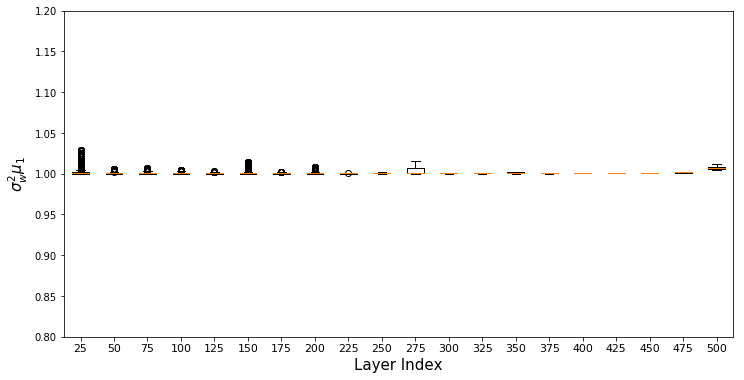
\includegraphics[width=1.0\textwidth]{img/supp/SuccBox}
    \caption
    [Box and whisker plot of $\sigma_w^2\mu_1$ for networks with successful training.]
    {Box and whisker plot of $\sigma_w^2\mu_1$ for networks with successful training. There are 18,579 successful runs.
    }
    \label{fig:succ_box}
\end{figure}

\begin{figure}[h]
    \centering
    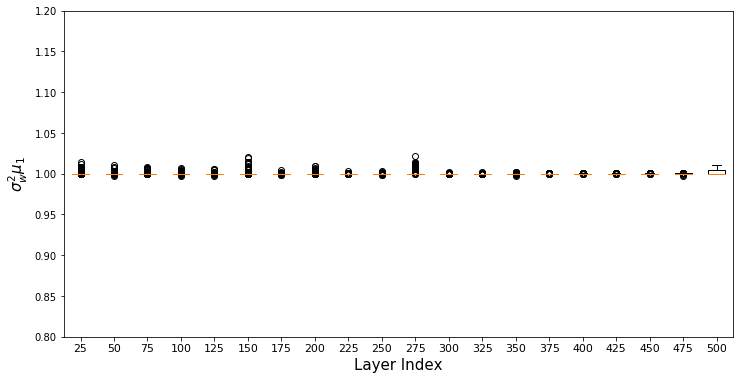
\includegraphics[width=1.0\textwidth]{img/supp/FailBox}
    \caption
    [Box and whisker plot of $\sigma_w^2\mu_1$ for networks with failed training.]
    {Box and whisker plot of $\sigma_w^2\mu_1$ for networks with failed training. There are 13,101 failed runs.
    }
    \label{fig:fail_box}
\end{figure}

\begin{figure}[h]
    \centering
    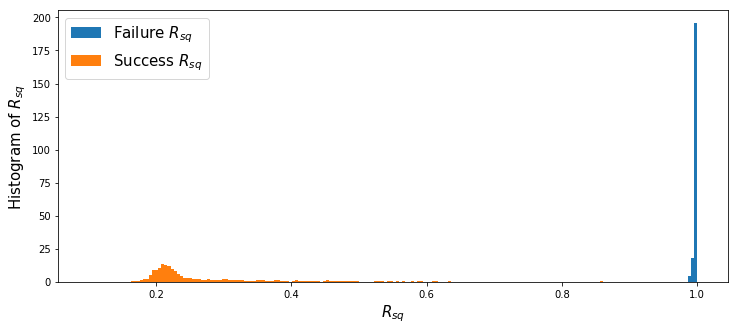
\includegraphics[width=1.0\textwidth]{img/supp/histogram}
    \caption{Histogram of $R_{sq}$ of failed/successful  networks.}
    \label{fig:histogram}
\end{figure}

\begin{table}[h]
    \centering
    \begin{tabular}{|c|c|c|r|r|}
    \hline
         Optimizer&Activation&Weight Init.&No. of Failure&No. of Success\\\hline
        
         \multirow{4}{*}{SGD}&Tanh&
         \multirow{2}{*}{Scaled Gaussian}&712&1268\\
         \cline{2-2}\cline{4-5}
         &ReLU&&1775&205\\\cline{2-5}
         &Tanh&\multirow{2}{*}{Orthogonal}&62&1918\\\cline{2-2}\cline{4-5}
         &ReLU&&882&1098\\\hline
         

         \multirow{4}{*}{SGD+momentum}&Tanh&\multirow{2}{*}{Scaled Gaussian}&982&998\\\cline{2-2}\cline{4-5}
         &ReLU&&1140&840\\\cline{2-5}
         &Tanh&\multirow{2}{*}{Orthogonal}&546&1434\\\cline{2-2}\cline{4-5}
         &ReLU&&1044&936\\\hline

         \multirow{4}{*}{Adam}&Tanh&\multirow{2}{*}{Scaled Gaussian}&609&1371\\\cline{2-2}\cline{4-5}
         &ReLU&&723&1257\\\cline{2-5}
         &Tanh&\multirow{2}{*}{Orthogonal}&354&1626\\\cline{2-2}\cline{4-5}
         &ReLU&&1465&515\\\hline
      
         \multirow{4}{*}{RMSProp}&Tanh&\multirow{2}{*}{Scaled Gaussian}&763&1217\\\cline{2-2}\cline{4-5}
         &ReLU&&827&1153\\\cline{2-5}
         &Tanh&\multirow{2}{*}{Orthogonal}&453&1527\\\cline{2-2}\cline{4-5}
         &ReLU&&764&1216\\\hline
    \end{tabular}
    \caption{The detailed numbers of successful and failed runs.}
    \label{num_table}
\end{table}
